\documentclass{standalone}
\usepackage{tikz}
\usetikzlibrary{patterns, positioning}
\usepackage[sfdefault]{ClearSans} %% option 'sfdefault' activates Clear Sans as the default text font
\usepackage[T1]{fontenc}

\begin{document}
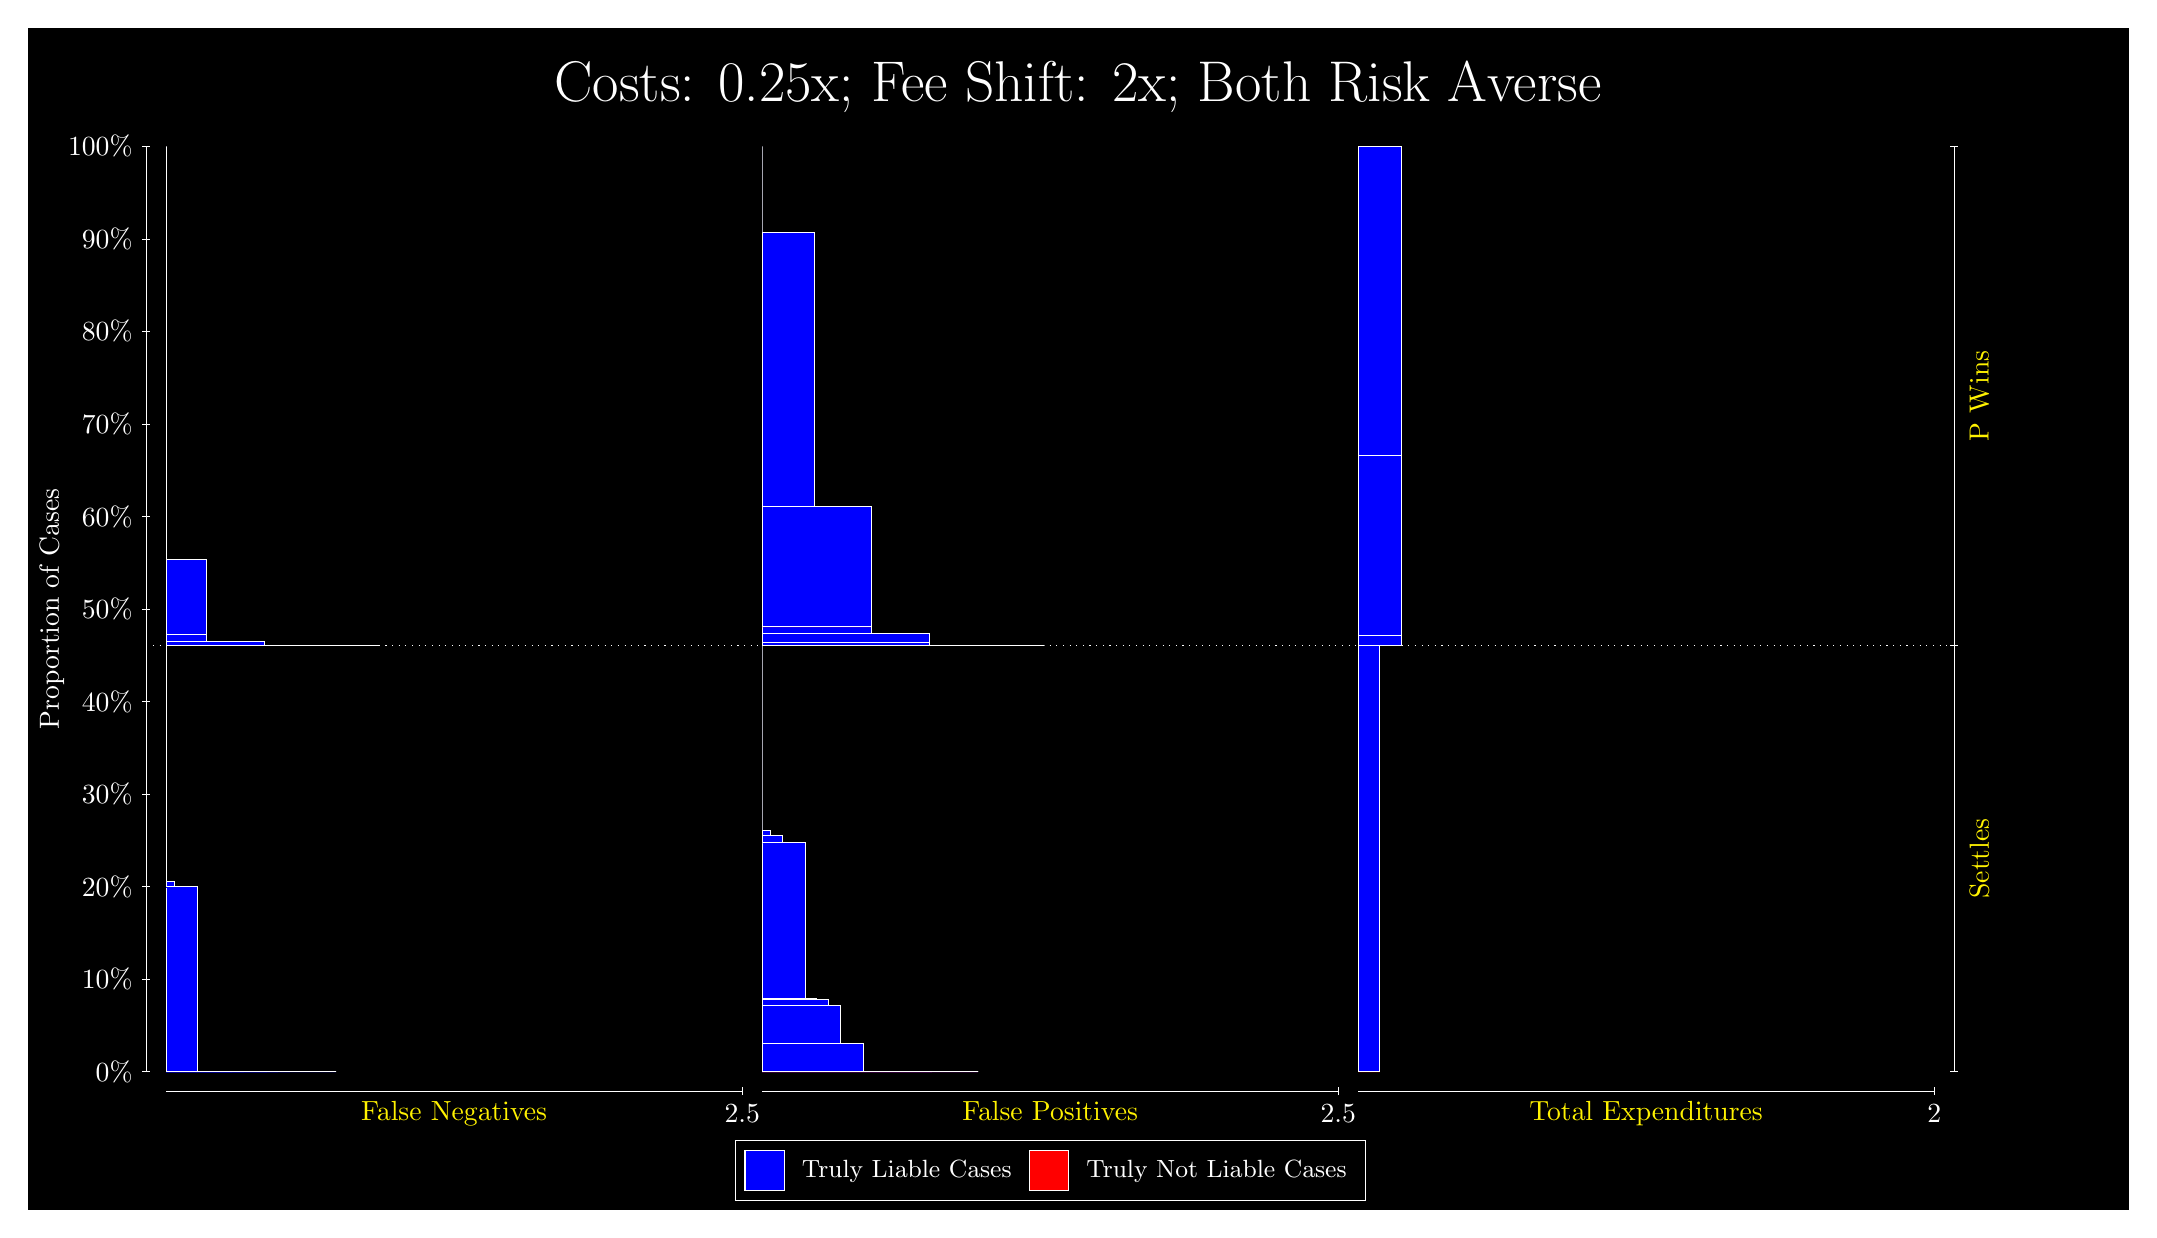
\begin{tikzpicture}
\draw[fill=black] (0,0) rectangle (26.667,15);
\draw[text=white] (0,13.5) rectangle (26.667,15) node[midway] {\huge Costs: 0.25x; Fee Shift: 2x; Both Risk Averse};
\draw[white, very thin] (1.5,1.75) -- (1.5,13.5);
\node[rotate=90, text=white, anchor=center] at (0.3, 7.625) {Proportion of Cases};
\draw[white, very thin] (1.45,1.75) -- (1.55,1.75);
\node[text=white, anchor=east] at (1.45, 1.75) {0\%};
\draw[white, very thin] (1.45,2.925) -- (1.55,2.925);
\node[text=white, anchor=east] at (1.45, 2.925) {10\%};
\draw[white, very thin] (1.45,4.1) -- (1.55,4.1);
\node[text=white, anchor=east] at (1.45, 4.1) {20\%};
\draw[white, very thin] (1.45,5.275) -- (1.55,5.275);
\node[text=white, anchor=east] at (1.45, 5.275) {30\%};
\draw[white, very thin] (1.45,6.45) -- (1.55,6.45);
\node[text=white, anchor=east] at (1.45, 6.45) {40\%};
\draw[white, very thin] (1.45,7.625) -- (1.55,7.625);
\node[text=white, anchor=east] at (1.45, 7.625) {50\%};
\draw[white, very thin] (1.45,8.8) -- (1.55,8.8);
\node[text=white, anchor=east] at (1.45, 8.8) {60\%};
\draw[white, very thin] (1.45,9.975) -- (1.55,9.975);
\node[text=white, anchor=east] at (1.45, 9.975) {70\%};
\draw[white, very thin] (1.45,11.15) -- (1.55,11.15);
\node[text=white, anchor=east] at (1.45, 11.15) {80\%};
\draw[white, very thin] (1.45,12.325) -- (1.55,12.325);
\node[text=white, anchor=east] at (1.45, 12.325) {90\%};
\draw[white, very thin] (1.45,13.5) -- (1.55,13.5);
\node[text=white, anchor=east] at (1.45, 13.5) {100\%};

\draw[white, very thin] (24.457,1.75) -- (24.457,13.5);
\draw[white, very thin] (24.407,1.75) -- (24.507,1.75);
\node[anchor=west] at (24.407, 1.75) {};
\draw[white, very thin] (24.407,7.1612) -- (24.507,7.1612);
\node[anchor=west] at (24.407, 7.1612) {};
\draw[white, very thin] (24.407,13.5) -- (24.507,13.5);
\node[anchor=west] at (24.407, 13.5) {};

\draw[white, very thin, fill=blue] (1.75,1.75) rectangle (3.9091,1.75);
\draw[white, very thin, fill=blue] (1.75,1.75) rectangle (3.3236,1.75);
\draw[white, very thin, fill=blue] (1.75,1.75) rectangle (3.1772,1.75);
\draw[white, very thin, fill=blue] (1.75,1.75) rectangle (3.0308,1.75);
\draw[white, very thin, fill=blue] (1.75,1.75) rectangle (2.738,1.75);
\draw[white, very thin, fill=blue] (1.75,1.75) rectangle (2.5917,1.7501);
\draw[white, very thin, fill=blue] (1.75,1.7501) rectangle (2.4453,1.7508);
\draw[white, very thin, fill=blue] (1.75,1.7508) rectangle (2.2989,1.7508);
\draw[white, very thin, fill=blue] (1.75,1.7508) rectangle (2.1525,4.097);
\draw[white, very thin, fill=blue] (1.75,4.097) rectangle (2.0062,4.0976);
\draw[white, very thin, fill=blue] (1.75,4.0976) rectangle (1.8598,4.1613);
\draw[white, very thin, fill=red] (1.75,4.1613) rectangle (1.75,4.1613);
\draw[white, very thin, fill=blue] (1.75,4.1613) rectangle (1.75,7.1612);
\draw[white, very thin, fill=blue] (1.75,7.1612) rectangle (4.458,7.1612);
\draw[white, very thin, fill=blue] (1.75,7.1612) rectangle (3.7261,7.1614);
\draw[white, very thin, fill=blue] (1.75,7.1614) rectangle (2.9942,7.1615);
\draw[white, very thin, fill=blue] (1.75,7.1615) rectangle (2.9942,7.2127);
\draw[white, very thin, fill=blue] (1.75,7.2127) rectangle (2.2623,7.3016);
\draw[white, very thin, fill=blue] (1.75,7.3016) rectangle (2.2623,8.2532);
\draw[white, very thin, fill=red] (1.75,8.2532) rectangle (1.75,8.2532);
\draw[white, very thin, fill=blue] (1.75,8.2532) rectangle (1.75,13.5);
\draw[white, very thin, fill=red] (9.3189,1.75) rectangle (12.063,1.75);
\draw[white, very thin, fill=blue] (9.3189,1.75) rectangle (12.063,1.75);
\draw[white, very thin, fill=red] (9.3189,1.75) rectangle (11.478,1.75);
\draw[white, very thin, fill=blue] (9.3189,1.75) rectangle (11.478,1.75);
\draw[white, very thin, fill=blue] (9.3189,1.75) rectangle (11.332,1.7524);
\draw[white, very thin, fill=red] (9.3189,1.7524) rectangle (11.185,1.7524);
\draw[white, very thin, fill=blue] (9.3189,1.7524) rectangle (11.185,1.7524);
\draw[white, very thin, fill=red] (9.3189,1.7524) rectangle (10.892,1.7524);
\draw[white, very thin, fill=blue] (9.3189,1.7524) rectangle (10.892,1.7533);
\draw[white, very thin, fill=blue] (9.3189,1.7533) rectangle (10.746,1.754);
\draw[white, very thin, fill=blue] (9.3189,1.754) rectangle (10.6,2.1119);
\draw[white, very thin, fill=blue] (9.3189,2.1119) rectangle (10.453,2.1121);
\draw[white, very thin, fill=red] (9.3189,2.1121) rectangle (10.307,2.1121);
\draw[white, very thin, fill=blue] (9.3189,2.1121) rectangle (10.307,2.5888);
\draw[white, very thin, fill=blue] (9.3189,2.5888) rectangle (10.161,2.6666);
\draw[white, very thin, fill=blue] (9.3189,2.6666) rectangle (10.014,2.6814);
\draw[white, very thin, fill=blue] (9.3189,2.6814) rectangle (9.8678,4.6574);
\draw[white, very thin, fill=blue] (9.3189,4.6574) rectangle (9.7214,4.6575);
\draw[white, very thin, fill=blue] (9.3189,4.6575) rectangle (9.575,4.75);
\draw[white, very thin, fill=blue] (9.3189,4.75) rectangle (9.4287,4.8136);
\draw[white, very thin, fill=blue] (9.3189,4.8136) rectangle (9.3189,7.1612);
\draw[white, very thin, fill=red] (9.3189,7.1612) rectangle (12.905,7.1612);
\draw[white, very thin, fill=blue] (9.3189,7.1612) rectangle (12.905,7.1612);
\draw[white, very thin, fill=blue] (9.3189,7.1612) rectangle (12.173,7.1622);
\draw[white, very thin, fill=red] (9.3189,7.1622) rectangle (12.173,7.1622);
\draw[white, very thin, fill=blue] (9.3189,7.1622) rectangle (12.173,7.1632);
\draw[white, very thin, fill=blue] (9.3189,7.1632) rectangle (11.441,7.206);
\draw[white, very thin, fill=red] (9.3189,7.206) rectangle (11.441,7.206);
\draw[white, very thin, fill=blue] (9.3189,7.206) rectangle (11.441,7.3116);
\draw[white, very thin, fill=blue] (9.3189,7.3116) rectangle (10.709,7.3993);
\draw[white, very thin, fill=red] (9.3189,7.3993) rectangle (10.709,7.3993);
\draw[white, very thin, fill=blue] (9.3189,7.3993) rectangle (10.709,8.9263);
\draw[white, very thin, fill=blue] (9.3189,8.9263) rectangle (9.9776,8.9288);
\draw[white, very thin, fill=red] (9.3189,8.9288) rectangle (9.9776,8.9288);
\draw[white, very thin, fill=blue] (9.3189,8.9288) rectangle (9.9776,12.408);
\draw[white, very thin, fill=blue] (9.3189,12.408) rectangle (9.3189,13.5);
\draw[white, very thin, fill=red] (16.888,1.75) rectangle (17.162,1.75);
\draw[white, very thin, fill=blue] (16.888,1.75) rectangle (17.162,7.1612);
\draw[white, very thin, fill=red] (16.888,7.1612) rectangle (17.437,7.1612);
\draw[white, very thin, fill=blue] (16.888,7.1612) rectangle (17.437,7.2951);
\draw[white, very thin, fill=red] (16.888,7.2951) rectangle (17.437,7.2951);
\draw[white, very thin, fill=blue] (16.888,7.2951) rectangle (17.437,9.5791);
\draw[white, very thin, fill=red] (16.888,9.5791) rectangle (17.437,9.5791);
\draw[white, very thin, fill=blue] (16.888,9.5791) rectangle (17.437,13.5);
\draw[white, dotted] (1.5,7.1612) -- (24.457,7.1612);
\draw[white, very thin] (1.75,1.5) -- (9.0689,1.5);
\node[text=yellow, anchor=north] at (5.4094, 1.5) {False Negatives};
\draw[white, very thin] (9.0689,1.45) -- (9.0689,1.55);
\node[text=white, anchor=north] at (9.0689, 1.45) {2.5};

\draw[white, very thin] (9.3189,1.5) -- (16.638,1.5);
\node[text=yellow, anchor=north] at (12.978, 1.5) {False Positives};
\draw[white, very thin] (16.638,1.45) -- (16.638,1.55);
\node[text=white, anchor=north] at (16.638, 1.45) {2.5};

\draw[white, very thin] (16.888,1.5) -- (24.207,1.5);
\node[text=yellow, anchor=north] at (20.547, 1.5) {Total Expenditures};
\draw[white, very thin] (24.207,1.45) -- (24.207,1.55);
\node[text=white, anchor=north] at (24.207, 1.45) {2};

\node[text=yellow, centered, rotate=90] at (24.777, 4.4556) {Settles};
\node[text=yellow, centered, rotate=90] at (24.777, 10.331) {P Wins};

\draw (12.978300999999998,1.5) node[draw=none] (baseCoordinate) {};
\begin{scope}[align=center]
        \matrix[scale=0.5, draw=white, below=0.5cm of baseCoordinate, nodes={draw}, column sep=0.1cm]{
            \node[rectangle, draw, minimum width=0.5cm, minimum height=0.5cm, fill=blue] {}; &
            \node[draw=none, font=\small, text=white] (B) {Truly Liable Cases}; &
            \node[rectangle, draw, minimum width=0.5cm, minimum height=0.5cm, fill=red] {}; &
            \node[draw=none, font=\small, text=white] (B) {Truly Not Liable Cases}; \\
            };
\end{scope}

\end{tikzpicture}
\end{document}